\section{Linguagem Java}
Java é considerada a linguagem de programação orientada a objetos mais utilizada no Mundo, ela é a base para construção de ferramentas como Hadoop, Pentaho, Weka e muitos outros utilizados comercialmente. Foi desenvolvida na década de 90 por uma equipe de programadores chefiada por \textit{James Gosling} para o projeto Green, na empresa Sun Microsystems - tornou-se nessa época como a linguagem que os programadores mais baixaram e o sucesso foi instantâneo. Em 2008 o Java foi adquirido pela empresa Oracle Corporation.

\subsection{Driver JDBC de Conexão}
Para proceder a conexão com Java, é necessário baixar um driver JDBC (Java Database Connection). Existem vários drivers construídos, porém o driver oficialmente suportado pelo MongoDB se encontra no endereço: \url{http://mongodb.github.io/mongo-java-driver}

Para utilizar o driver é necessário criar um projeto (vamos usar o \textbf{Spring Tool Suite 4}, utilize se quiser qualquer outro editor de sua preferência).

No STS4 acessar a seguinte opção no menu: File $\triangleright$ New $\triangleright$ Java Project. Informar o nome do projeto, não esquecer de modificar a opção "Use an environment JRE" para a versão correta da Java Runtime desejada e pressionar o botão Finish. Se está tudo correto teremos a seguinte situação na aba \textit{Project Explorer}:
\begin{figure}[H]
	\centering
	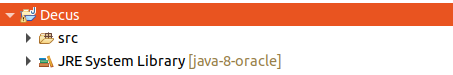
\includegraphics[width=0.5\textwidth]{imagens/projetoCriado.png}
	\caption{Projeto Decus criado}
\end{figure}

Vamos convertê-lo para um projeto Apache Maven. Clicar com o botão direito do mouse no projeto e acessar a opção: Configure $\triangleright$ Convert to Maven Project. Na janela apenas pressione o botão \textit{Finish}. Se tudo está correto observamos que o projeto ganhou uma letra \textbf{M} o que indica agora é um projeto padrão Maven. Então foi criado um arquivo chamado \textbf{pom.xml}. 

Acessar este arquivo e antes da tag BUILD, inserir a tag DEPENDENCIES:
\begin{lstlisting}[]
<dependencies>
  <!-- Logging -->
  <dependency>
    <groupId>org.slf4j</groupId>
    <artifactId>slf4j-simple</artifactId>
    <version>1.7.5</version>
  </dependency>
  <dependency>
    <groupId>org.slf4j</groupId>
    <artifactId>slf4j-log4j12</artifactId>
    <version>1.7.5</version>
  </dependency>
  <dependency>
    <groupId>org.slf4j</groupId>
    <artifactId>slf4j-api</artifactId>
    <version>1.7.5</version>
  </dependency>
  <!-- Driver Banco MongoDB -->
  <dependency>
    <groupId>org.mongodb</groupId>
    <artifactId>mongodb-driver-sync</artifactId>
    <version>4.0.4</version>
  </dependency>
</dependencies>
\end{lstlisting}

Agora a situação do projeto é esta:
\begin{figure}[H]
	\centering
	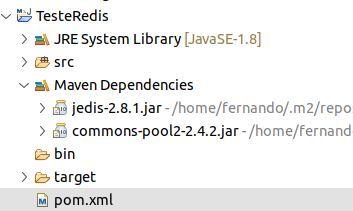
\includegraphics[width=0.6\textwidth]{imagens/dependenciasMaven.png}
	\caption{Dependências do Maven}
\end{figure}

Observamos que na pasta \textbf{Maven Dependencias} foi baixado a versão 4.0.4 do driver MongoDB.

\subsection{Testar a Conexão}
Estamos prontos para testarmos a conexão entre MongoDB e Java. Vamos criar um pequeno exemplo que nos auxiliará como teste devemos criar uma classe chamada \textbf{Escola} no pacote \textbf{decus.com} e inserir nesta a seguinte codificação:
\begin{lstlisting}[]
package decus.com;
	
import org.bson.Document;
import com.mongodb.client.MongoClients;
import com.mongodb.client.MongoClient;
import com.mongodb.client.MongoDatabase;
import com.mongodb.client.MongoCollection;
import com.mongodb.client.MongoCursor;
	
public class Escola {
  private MongoDatabase db;
  private MongoClient mongo;
  private MongoCollection<Document> col;
		
  protected MongoDatabase getDb() {
    return db;
  }
  protected MongoCollection<Document> getCol() {
    return col;
  }
		
  protected MongoClient getMongo() {
    return mongo;
  }
		
  protected boolean conectar() {
    try {
      mongo = MongoClients.create("mongodb://localhost:27017");
      db = mongo.getDatabase("escola");
      col = db.getCollection("aluno");
    } catch (Exception e) {
      return false;
    }
    return true;
  }
		
  protected boolean desconectar() {
    try {
      mongo.close();
    } catch (Exception e) {
      return false;
    }
    return true;
  }
		
  private void executar() {
    if (this.conectar()) {

      // Inserir os alunos
      Document doc = new Document("nome", "Mario da Silva").append("nota", (int)(Math.random() * 10));
      col.insertOne(doc);
      doc = new Document("nome", "Aline Moraes").append("nota", (int)(Math.random() * 10));
      col.insertOne(doc);
      doc = new Document("nome", "Soraya Gomes").append("nota", (int) (Math.random() * 10));
      col.insertOne(doc);
				
      // Listar os Alunos
      MongoCursor<Document> cursor = col.find().iterator();
      while (cursor.hasNext()) {
        doc = cursor.next();
        System.out.println(doc.get("nome") + ": " + doc.get("nota"));
      }
      cursor.close();
      this.desconectar();
    }
  }
		
  public static void main(String[] args) {
    new Empresa().executar();
  }
}
\end{lstlisting}

Esta classe adiciona três registros ao banco de dados contendo o nome do aluno e sua nota que é gerada de forma randômica e em seguida procede uma consulta para verificar se os registros foram realmente inseridos. A conexão e desconexão ao MongoDB foi colocada em métodos separados.

No Shell utilizar os seguintes comandos para verificar os dados:
\begin{lstlisting}[]
> show dbs
> use escola
> show collections
> db.aluno.find()
\end{lstlisting}

E se tudo está OK, teremos o seguinte resultado:
\begin{figure}[H]
	\centering
	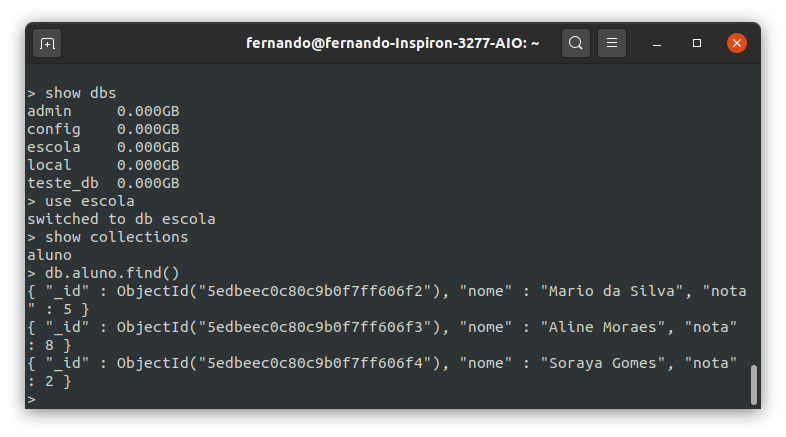
\includegraphics[width=0.6\textwidth]{imagens/testeOK.png}
	\caption{Execução do Shell}
\end{figure}

\subsection{Programação Java usando o MongoDB}
Nesta seção será visto como via linguagem Java é possível gerenciar os objetos do MongoDB. Os comandos dos exemplos a seguir foram escritos a partir dos objetos existentes no código anterior. Por esse motivo deixamos os métodos protegidos ao invés de particulares e criamos os tipo \textit{GET} para objetos que estão na mesma classe.

Criar uma nova classe chamada \textbf{TstComando}, que estende a classe \textbf{Escola} no mesmo pacote com a seguinte codificação:
\begin{lstlisting}[]
package decus.com;
	
public class TstComando extends Escola {
  public static void main(String[] args) {
    new TstComando().executar();
  }

  private void executar() {
    if (conectar()) {
      // Inserir o comando aqui
      desconectar();
    }
  }
}
\end{lstlisting}

Esta classe agora será a nossa principal, sendo assim removemos os métodos \textbf{main} e \textbf{executar} da classe \textbf{Escola} que já serviram a seu propósito. Lembre-se que a Programação Orientada a Objetos é uma metodologia e não uma linguagem, se pratica essa forma ao usarmos os princípios da Orientação a Objetos e aproveitar a qualidade de extensibilidade do código.

\subsection{Informações dos Documentos}
Para obter informações dos documentos, é possível utilizar diversas ações. 

Listar as bases de dados existentes: \\
\codigo{ for (String s: getMongo().listDatabaseNames()) \{ \\
	\phantom{x}\hspace{4pt} System.out.println(s); \\
	\} }

Criar uma nova coleção na base de dados pelo seu nome: \\
\codigo{ MongoDatabase db2 = getMongo().getDatabase("escola");}

Verificar quais são as coleções existentes em uma determinada base de dados: \\
\codigo{ for (String s: getDb().listCollectionNames()) \{ \\
	\phantom{x}\hspace{4pt} System.out.println(s); \\
	\}}

Criar uma nova coleção pelo seu nome e através deste obter a quantidade de documentos existentes: \\
\codigo{ MongoCollection<Document> col2 = getDb().getCollection("aluno"); \\
	System.out.println("Total de Documentos:" + col2.countDocuments());}

Obter, em formato JSON (\textit{JavaScript Object Notation}), as coleções de uma determinada base de dados: \\
\codigo{ ListCollectionsIterable<Document> it = getDb().listCollections(); \\
	MongoCursor<Document> cursor = it.iterator(); \\
	while (cursor.hasNext()) \{ \\
	\phantom{x}\hspace{4pt} System.out.println(cursor.next().toJson()); \\
	\} \\
	cursor.close();}

Criar um índice para uma coleção, o parâmetro com valor igual a 1 informa que deve ser ordenado de forma ascendente (descendente utilizamos o valor -1): \\
\codigo{ getCol().createIndex(new Document("nota", 1));}

Obter, em formato JSON, os índices de uma determinada coleção: \\
\codigo{ ListIndexesIterable<Document> it = getCol().listIndexes(); \\
	MongoCursor<Document> cursor = it.iterator(); \\
	while (cursor.hasNext()) \{ \\
	\phantom{x}\hspace{4pt} System.out.println(cursor.next().toJson()); \\
	\} \\
	cursor.close();}

Eliminar um indice de uma coleção: \\
\codigo{ getCol().dropIndex(new Document("nota", 1));}

Obter, em formato JSON, os documentos de uma determinada coleção: \\
\codigo{ MongoCursor<Document> cursor = getCol().find().iterator(); \\
	while (cursor.hasNext()) \{ \\
	\phantom{x}\hspace{4pt} System.out.println(cursor.next().toJson()); \\
	\} \\
	cursor.close();}

Para os próximos exemplo, consideraremos o método executar() conforme o código abaixo e procedemos a inserção do comando descrito na posição indicada:
\begin{lstlisting}[]
private void executar() {
  if (conectar()) {
    // Inserir o comando aqui
    while (cursor.hasNext()) {
      System.out.println(cursor.next().toJson());
    }
    cursor.close();  
    desconectar();
  }
}
\end{lstlisting}

\subsection{Filtrar Coleções}
Limitar a quantidade de documentos retornados (por exemplo 2): \\
\codigo{ MongoCursor<Document> cursor = getCol().find().limit(2).iterator();}

Trazer os alunos que obtiveram nota 10: \\
\codigo{ MongoCursor<Document> cursor = getCol().find(new Document("nota", 10)).iterator();}

Através da classe \texttt{com.mongodb.client.model.Filters} é possível realizar a mesma ação: \\
\codigo{ MongoCursor<Document> cursor = getCol().find(Filters.eq("nota", 10)).iterator();}

E com a utilização dessa classe, é possível realizar as seguintes ações:
\begin{itemize}[nolistsep]
	\item \textbf{Filters.ne} - registros não iguais a um determinado valor
	\item \textbf{Filters.gt} - registros maiores que um determinado valor
	\item \textbf{Filters.gte} - registros maiores ou iguais a um determinado valor
	\item \textbf{Filters.lt} - registros menores que um determinado valor
	\item \textbf{Filters.lte} - registros menores ou iguais a um determinado valor
\end{itemize}

Para realizar a mesma consulta com a utilização dos filtros: \\
\codigo{ MongoCursor<Document> cursor = getCol().find( \\
	Filters.and(Filters.gt("nota", 3), Filters.lt("nota", 9))).iterator();}

Também podemos utilizar as variáveis: 
\begin{itemize}[nolistsep]
	\item \$eq - Igual
	\item \$ne - Não igual
	\item \$gt - Maior
	\item \$gte - Maior ou igual
	\item \$lt - Menor
	\item \$lte - Menor ou igual. 
\end{itemize}

Obter todos os documentos da coleção com a nota é maior que 6: \\
\codigo{ MongoCursor<Document> cursor = getCol().find( \\
	new Document("nota", new  Document("\$gt",6))).iterator(); } 

Parece mais complicado, porém é possível criar separadamente um objeto Documento e a partir dele compor combinações. Obter todos os documentos cujas notas são maiores que 3 e menores que 9: \\
\codigo{ Document doc = new Document(); \\
	doc.append("nota", new Document("\$gt", 3).append("\$lt", 9)); \\
	MongoCursor<Document> cursor = getCol().find(doc).iterator();}

\subsection{Ordenações}
Através da classe \texttt{com.mongodb.client.model.Sorters}, e podemos utilizar as variáveis ``ascending'' e ``descending'' para obter ordenações: \\
\codigo{ MongoCursor<Document> cursor = \\
	col.find().sort(Sorts.ascending("nota")).iterator();}

\section{Modificar os documentos da Coleção via Java}
Uma vez identificado o(s) documento(s) desejado(s) é possível proceder:
\begin{itemize}[nolistsep]
	\item Alterações. Utilizar os métodos updateOne ou updateMany.
	\item Eliminações. Utilizar os métodos deleteOne ou deleteMany.
\end{itemize}

Modificar a nota do aluno ``Mario da Silva'' para 5: \\
\codigo{ getCol().updateOne(new Document("nome","Mario da Silva"), \\
	new Document("\$set", new Document("nota", 5))); }

Para eliminar o aluno ``Mario da Silva'': \\
\codigo{ getCol().deleteMany(new Document("nome","Mario da Silva"));}

\subsection{Eliminar os documentos}
Para eliminar a coleção ``aluno'': \\
\codigo{ getCol().drop(); }

Para eliminar a base de dados ``escola'': \\
\codigo{ getDb.drop();}
